% Section 3: System Design

\subsection{Method Overview}
\label{sec:system:overview}

\epikg implements three key ideas: (1)~end-to-end epistemic preservation, carrying assertion labels from NLP extraction through OMOP mapping, fact construction, KG materialization, and retrieval; (2)~tri-temporal edge representation, storing valid time, transaction time, and NLP-asserted temporality on every KG edge; and (3)~intent-aware routing, matching graph traversal strategy to question type.
The first two ideas are necessary infrastructure; the third is where the performance gain originates.
The key invariant is that \textit{epistemic assertion status} is a first-class attribute at every stage, not an NLP annotation discarded after extraction (Figure~\ref{fig:architecture}).
Clinical concepts are stored once as shared global nodes; patient-specific semantics (assertion status, temporality, confidence) reside on edges.

\begin{figure}[t]
\centering
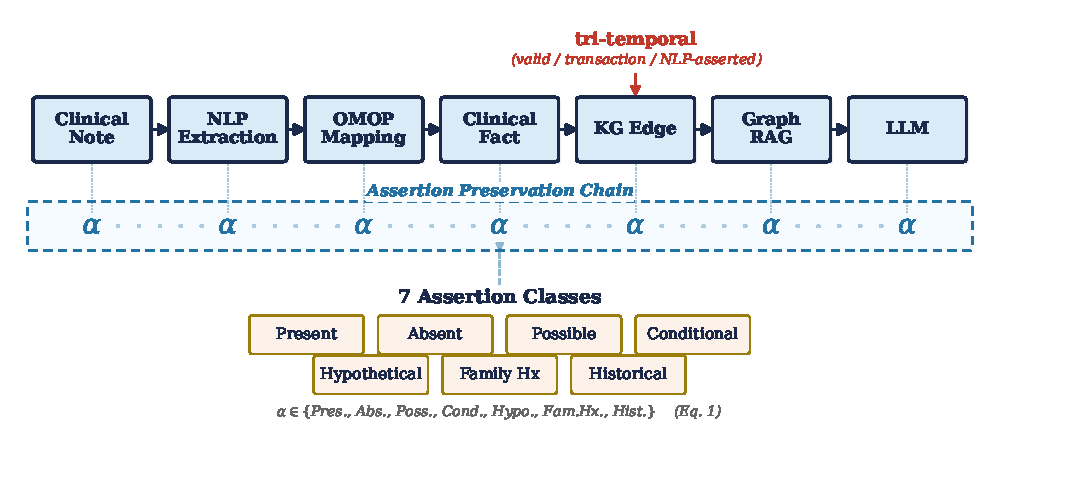
\includegraphics[width=\textwidth]{figures/fig1_architecture.pdf}
\caption{The \epikg pipeline. The assertion label $\alpha$ (highlighted) is preserved as a first-class attribute from NLP extraction through OMOP mapping, fact construction, KG materialization, and assertion-aware GraphRAG.}
\label{fig:architecture}
\end{figure}

\subsection{Epistemic Assertion Schema}
\label{sec:system:assertion}

\looseness=-1
Clinical notes abound with qualified statements---``\textit{no evidence of pneumonia},'' ``\textit{possible CHF},'' ``\textit{mother had breast cancer}''---yet standard representations discard these qualifiers.
OMOP excludes negated conditions entirely~\cite{omop2024}; FHIR limits assertion metadata to conditions.
\epikg defines a seven-value assertion taxonomy:
%
\begin{equation}
\label{eq:assertion}
\alpha \in \{\text{\scriptsize Pres., Abs., Poss., Cond., Hypo., Fam.Hx., Hist.}\}
\end{equation}
%
This extends the i2b2 six-class taxonomy~\cite{uzuner2011i2b2assertion} by separating \textsc{Historical} from \textsc{Family\_History}, a clinically important distinction that prior work conflates (definitions in Appendix~\ref{app:assertions}).
A rule-based classifier (122 scope-aware trigger patterns) assigns $\alpha$ with an associated confidence score.
The label is carried through every stage: from \texttt{ExtractedMention} through ensemble merging, \texttt{ClinicalFact} records, KG edge properties, and retrieval scoring.
Additionally, each edge carries a tri-temporal representation---valid time, transaction time, and NLP-asserted temporality---with Allen-style interval relations as first-class retrieval features (formalized in Appendix~\ref{app:temporal_model}).

\subsection{Formal Epistemic Preservation}
\label{sec:system:formal}

We formalize the epistemic invariant maintained by the \epikg pipeline, building on the ontological principle that aboutness must be preserved across transformations~\cite{ceusters2015ontologyepistemology}.
The \emph{epistemic state} of a clinical mention $m$ is the tuple $e(m) = (c, \alpha, \xi, \tau)$: OMOP concept, 7-value assertion label, experiencer ($\{\textsc{Patient}, \textsc{Family}\}$), and temporality ($\{\textsc{Current}, \textsc{Past}, \textsc{Future}\}$); see Table~\ref{tab:notation} (Appendix) for notation summary.
A pipeline \emph{epistemically preserves} $m$ if the output epistemic state equals the extraction state at every stage.
We formalize (Appendix~\ref{app:formal}) that an assertion-blind pipeline collapses the assertion distribution to a degenerate point mass, incurring entropy loss $\Delta H = H(A_c^\pi) \geq 0$~\cite{shannon1948}, and that assertion-faithful accuracy is bounded by $1 - f_{\textit{np}}(c)$, where $f_{\textit{np}}$ is the fraction of non-present assertions.
The empirical consequences are measured via category-stratified accuracy in Section~\ref{sec:results}.


\subsection{Intent-Aware Retrieval (C4g)}
\label{sec:system:intentaware}

The base retrieval pipeline uses bidirectional BFS over patient KG edges and OMOP vocabulary relationships (details in Appendix~\ref{app:retrieval_details}), but treats all questions uniformly.
Yet different clinical question types require fundamentally different graph operations.
A \emph{change} question requires cross-admission set differencing; a \emph{current-state} question needs filtering to the most recent valid edges; a \emph{historical} question must recover resolved conditions.

\paragraph{Intent classifier.}
A lightweight rule-based classifier maps each question to one of four intents---\textsc{Change}, \textsc{Current\_State}, \textsc{Historical}, or \textsc{Default}---using question metadata with keyword-pattern fallback (Algorithm~\ref{alg:c4g}, Appendix~\ref{app:routing}).

\paragraph{Change retrieval.}
For $\iota = \textsc{Change}$, edges are partitioned by admission (\texttt{hadm\_id}).
The module computes set differences across admission pairs $(k, k')$---concepts \emph{added} ($\mathcal{C}_{k'} \!\setminus\! \mathcal{C}_k$), \emph{removed} ($\mathcal{C}_k \!\setminus\! \mathcal{C}_{k'}$), and \emph{continued} ($\mathcal{C}_k \!\cap\! \mathcal{C}_{k'}$)---and returns structured evidence.

\paragraph{Current-state and historical retrieval.}
For \textsc{Current\_State}, the module filters to edges with $\tau_a = \textsc{Current}$ or open-ended validity, deduplicates by concept, and emits ``\textsc{Not Found}'' for missing concepts.
For \textsc{Historical}, it selects edges with $\tau_a = \textsc{Past}$ and augments with admission-based inference (concepts in earlier admissions but absent from the latest are labeled ``resolved'').
Each intent triggers a type-specific prompt template that structures evidence according to question semantics (Appendix~\ref{app:example}).
